\chapter{Development of the first GRB search in ANITA constrained in direction and time}
\label{grb_technique}

\section{Gamma Ray Bursts during the ANITA-3 flight}

The IceCube catalog was used to determine which \gls{grbs} took place during the third flight of \gls{anita}. The catalog provides information such as the \gls{grb} name, which day the \gls{grb} occurred, the time of trigger in UTC, the time over which a burst emits from 5\% of its total measured counts to 95\%, the \gls{ra}, and the \gls{dec}, among other properties. There were 18 \gls{grbs} during \gls{anita}-3. Relevant information on these \gls{grbs} as obtained from the catalog are shown in Table~\ref{catalog}. 

Table~\ref{info_found} shows information on the \gls{grbs} that was either calculated or found in data. 
The ``Catalog UT" column shows the unixtime calculated for each \gls{grb} using the date and time provided by the catalog (code in Figure~\ref{unixtime_code}). ``Closest recorded UT" is the closest unixtime recorded by \gls{anita} corresponding to the unixtime calculated from the catalog. It can be seen that this closest recorded unixtime is the same as the catalog unixtime for all except one \gls{grb}. GRB141225A took place on December 25, 2014 which is when the \gls{anita}-3 flight was temporarily out of commission due to technical problems, therefore, the closest recorded unixtime for this \gls{grb} is not identical to the catalog unixtime. Also shown in Table~\ref{info_found}, are the run number that corresponds to each \gls{grb} unixtime, and the longitude, latitude, and altitude of the \gls{anita} payload at that time. Longitude and latitude are shown in degrees. Altitude is in meters. 

\begin{table}
\centering
\begin{tabular}{ |c|c|c|c|c|c| } 
\hline
GRB name & Date & UTT (Trigger) & T90 & RA & Dec\\
\hline
141220A	& 12-20-14  & 6:02:51   & 8.448	& 195.058 & 32.146\\
141221A	& 12-21-14	& 8:07:10   & 36.9	& 198.287 & 8.205\\
141221B	& 12-21-14	& 21:31:48	& 32.51	& 126.02  &	-74.21\\
141222A	& 12-22-14	& 7:08:55	& 8.448	& 178.04  &	-57.35\\
141222B	& 12-22-14	& 16:34:30	& 34.05	& 97.43	  & 40.13\\
141223A	& 12-23-14	& 5:45:37	& 94.2	& 147.38  &	-20.71\\
141225A	& 12-25-14	& 23:01:13	& 56.32	& 138.778 &	33.792\\
141226A	& 12-26-14	& 21:07:24	& 38.65	& 163.85  &	28.39\\
141229A	& 12-29-14	& 11:48:59	& 13.82	& 71.479  &	-18.956\\
141229B	& 12-29-14	& 21:52:10	& 22.02	& 170.1	  & 23.06\\
141230A	& 12-30-14	& 3:24:22	& 9.86	& 56.98	  & 1.59\\
141230B	& 12-30-14	& 20:00:25	& 28.93	& 181.47  &	11.65\\
141230C	& 12-30-14	& 20:54:05	& 0.22	& 246.93  &	-40.18\\
150101A	& 01-01-15	& 6:28:53	& 0.24	& 312.603 &	36.733\\
150101B	& 01-01-15	& 15:23:34	& 0.08	& 188.0	  & -10.956\\
150103A	& 01-03-15	& 20:02:18	& 49.1	& 131.666 &	-48.886\\
150105A	& 01-05-15	& 6:10:00	& 73.73	& 124.32  &	-14.78\\
150106A	& 01-06-15	& 22:05:56	& 79.88	& 40.83	  & 0.31\\
\hline
\end{tabular}
\caption{Information from the IceCube catalog on the Gamma Ray Bursts that took place during the ANITA-3 flight. T90 is in seconds. RA and Dec are in degrees.}
\label{catalog}
\end{table}

\begin{table}
\centering
\begin{tabular}{ |c|c|c|c|c|c|c| } 
\hline
GRB & Catalog UT & Closest recorded UT & Run & Pl. Lon & Pl. Lat & Pl. Alt\\
\hline
141220A & 1419055371 & 1419055371 & 175 & 126.3 & -82.0 & 36215.0\\
141221A & 1419149230 & 1419149230 & 192 & 104.5 & -80.7 & 36602.1\\
141221B & 1419197508 & 1419197508 & 200 & 90.6 & -80.0 & 35001.6\\
141222A & 1419232135 & 1419232135 & 207 & 80.4 & -80.2 & 36680.9\\
141222B & 1419266070 & 1419266070 & 212 & 71.1 & -80.3 & 35927.8\\
141223A & 1419313537 & 1419313537 & 219 & 59.5 & -79.4 & 36609.9\\
141225A & 1419548473 & \color{red} {1419542007} & 256 & 8.1 & -78.5	& 35701.9\\
141226A & 1419628044 & 1419628044 & 272 & -11.8 & -78.4 & 36456.3\\
141229A & 1419853739 & 1419853739 & 308 & -62.1 & -78.5 & 36240.1\\
141229B & 1419889930 & 1419889930 & 313 & -69.3 & -78.9 & 36860.6\\
141230A & 1419909862 & 1419909862 & 316 & -68.7 & -78.5 & 35935.1\\
141230B & 1419969625 & 1419969625 & 324 & -82.1 & -78.1 & 36999.1\\
141230C & 1419972845 & 1419972845 & 324 & -82.3 & -78.1 & 36903.9\\
150101A & 1420093733 & 1420093733 & 341 & -106.5 & -76.1 & 34812.8\\
150101B & 1420125814 & 1420125814 & 345 & -114.1 & -76.5 & 36160.5\\
150103A & 1420315338 & 1420315338 & 371 & -159.3 & -74.6 & 36762.1\\
150105A & 1420438200 & 1420438200 & 389 & 169.9 & -74.5 & 37034.5\\
150106A & 1420581956 & 1420581956 & 409 & 129.7 & -72.9 & 35453.3\\
\hline
\end{tabular}
\caption{Information that I calculated or found in the data for each GRB during the ANITA-3 flight. Note that the longitude, latitude, and altitude are for the ANITA payload. Longitude and latitude are in degrees. Altitude of ANITA is in meters.}
\label{info_found}
\end{table}


\begin{figure}
\centering
%\begin{verbatim}
\begin{verbbox}
def main():
  datetimelist = numpy.zeros((rows, columns))
  datetimelist = [["2014,12,20","6:02:51"],..]
  for i in range(rows):
    stringdate = datetimelist[i][0]
    stringtime = datetimelist[i][1]
    objectdate = date(*map(int, (stringdate.split(","))))
    assert objectdate == 
    datetime.datetime.strptime(stringdate, "%Y,%m,%d").date()
    unixtime = calendar.timegm(objectdate.timetuple())
    timeseconds = sum(int(x) * 60 ** i 
    for i,x in enumerate(reversed(stringtime.split(":"))))
    unixtime = unixtime + timeseconds
main()
\end{verbbox}
\fbox{\theverbbox}
%\end{verbatim}
\caption{Code to calculate unixtime of each GRB from date and time from the catalog. This produced the ``Catalog UT" shown in Table~\ref{info_found}.}
\label{unixtime_code}
\end{figure}


\subsection{GRB direction: elevation angle and azimuth}

To determine the relevant direction associated with each \gls{grb}, it is necessary to calculate the altitude or elevation angle, and azimuth of each \gls{grb} with respect to the \gls{anita} payload. This can be done by utilizing the date, time, \gls{ra}, and \gls{dec} of each \gls{grb}, as provided by the catalog, and the longitude, latitude, and altitude of the \gls{anita} payload (the observer) at the time of each \gls{grb}. 
In other words, the elevation angle and azimuth can be calculated for each \gls{grb} using a combination of the information presented in Tables~\ref{catalog} and~\ref{info_found}. 
%Obtaining the correct elevation angle and azimuth is critical as the analysis to search for neutrinos from \gls{grbs} depends on the \gls{grb} directions, therefore, all information required to calculate these angles is presented in this chapter for cross-checking. 
The elevation angle and azimuth are calculated for each \gls{grb} using the Python code shown in Figure~\ref{alt_az_code}.
The calculated elevation angles and azimuths are presented in Table~\ref{alt_az}. 
%Note that these angles need to be adjusted to be consistent with the coordinate system of iceMC for elevation angle and azimuth, as discussed in Section~\ref{grb_sim}. 

\begin{table}
\centering
\begin{tabular}{ |c|c|c| } 
\hline
GRB & Azimuth (degrees) & Elevation angle (degrees)\\
\hline
141220A	& 254.48 & -34.54\\
\color{red} {141221A}	& 243.88 & -12.34 \\
141221B	& 316.33 & 83.06\\
141222A	& 245.82 & 54.49\\
141222B	& 41.79 & -33.14\\
141223A	& 266.01 & 20.41\\
141225A	& 46.19 & -26.10\\
141226A	& 117.67 & -34.25\\
\color{red} {141229A}	& 216.78 & 9.78 \\
141229B	& 172.51 & -34.02\\
\color{red} {141230A}	& 336.03 & 8.84 \\
141230B	& 226.89 & -19.92\\
141230C	& 266.61 & 40.56\\
150101A	& 230.28 & -46.49\\
150101B	& 328.30 & 22.67\\
150103A	& 233.77 & 41.27\\
\color{red} {150105A}	& 120.18 & 7.33 \\
150106A	& 194.23 & -16.95\\
\hline
\end{tabular}
\caption{Elevation angle and azimuth of each GRB during the ANITA-3 flight. Note that these angles need to be adjusted to be consistent with the coordinate system of icemc for elevation angle and azimuth. Technique for finding these angles has been verified using the case of mystery event 2.}
\label{alt_az}
\end{table}

\begin{figure}
\centering
\begin{verbbox}
from astropy.coordinates import EarthLocation, SkyCoord, AltAz
from astropy.time import Time
from astropy import units as u
from astropy.coordinates import AltAz

def main():

  grb_list = pd.read_csv
  ('/Users/oindreebanerjee/python/A3_GRB_List_For_Astropy.csv')

  for i in range(0,grb_list.shape[0]):
  
    Anita_location = EarthLocation(lon = grb_list.loc[: ,
    "ANITA_Longitude_Begin"][i], lat = 90 + grb_list.loc[: ,
    "ANITA_Latitude_Begin"][i], height = grb_list.loc[: ,
    "ANITA_Altitude_Begin"][i] * u.m)

    time_string = grb_list.loc[: , "Date"][i] + " " 
    + grb_list.loc[: , "Time"][i]

    grb_time = Time(time_string)

    Anita_frame = AltAz(location = Anita_location, 
    obstime = grb_time)

    coord = SkyCoord(grb_list.loc[: , "GRB_RA"][i] * u.degree,
    grb_list.loc[: , "GRB_Dec"][i] * u.degree)

    coordAnita = coord.transform_to(Anita_frame)
    
main()
\end{verbbox}
\fbox{\theverbbox}
\caption{Code to calculate elevation angle and azimuth of each GRB. This produced the angles shown in Table~\ref{alt_az}.}
\label{alt_az_code}
\end{figure}


\subsubsection{Verification of angles}

To verify that I am calculating the correct elevation angles and azimuths for the \gls{grbs}, I used known information on a special event from \gls{anita}-3, known as the mystery event 2~\cite{me2}. The event number for this event is 15717147. 
The relevant information on mystery event 2 is shown in Table~\ref{me2_verify}. Using these as inputs, I calculated the elevation angle and azimuth of the mystery event 2. I got -35.0 degrees for elevation angle and 61.6 degrees for azimuth which match what was found in~\cite{me2}. The \gls{grb} angles shown in Table~\ref{alt_az} were calculated using the same method so these should be correct as well. 

\begin{table}
\centering
\begin{tabular}{ |c|c|c|c|c|c|c| } 
\hline
RA & Dec & Pl. Lon & Pl. Lat & Pl. Alt & Date & Time\\
\hline
50.78203 &	38.65498 &	126.5 &	-81.6 &	35861.0 &	
2014-12-20 & 8:33:22\\
\hline
\end{tabular}
\caption{Info on mystery event 2. The longitude, latitude, and altitude reported here are that of the ANITA payload during the event.}
\label{me2_verify}
\end{table}


\subsection{Selecting GRBs for the search}

Initially, only the \gls{grbs} shown in red font in Table~\ref{alt_az} were selected for the purpose of performing a binned search for \gls{grb} neutrinos. The reason behind this selection is based on the distribution of elevation angles shown in Figure~\ref{nuDir_kotera_isotropic}. A distribution of elevation angles of weighted simulated neutrinos using an isotropic Kotera flux is shown in Figure~\ref{nuDir_kotera_isotropic}. This shows that most simulated neutrinos viewable by \gls{anita} have elevation angles that are within a range of about -15 to about 12 degrees. Therefore, the \gls{grbs} with elevation angles of -12.34, 9.78, 8.84, and 7.33 degrees were initially selected for the search.

\subsubsection{Mystery-event-like elevation angles}

There are several \gls{grbs} in the sample shown in Table~\ref{alt_az} that have elevation angles similar to that of the mystery event observations reported by \gls{anita} in~\cite{me1,me2}. In general, such a signal that involves a steep elevation angle like that of the mystery events is not expected to be detected via the Askaryan Effect. Both mystery events were observed utilizing their geomagnetic radiation due to associated air showers. Such signals are expected to have a strong \gls{hpol} content and typically regarded as cosmic ray signatures, although in the case of the mystery events, the origin of the events is still under study. To accommodate mystery-event-like elevation angles, the \gls{grbs} with steeper elevation angles were also included. 

At that point, few \gls{grbs} remained with elevation angles above the horizon. These were also included in the search, although the geometry associated with them would be challenging for detection. To summarize, all 18 \gls{grbs} were included in the search for \gls{uhe} neutrinos. 

\begin{figure}
\centering
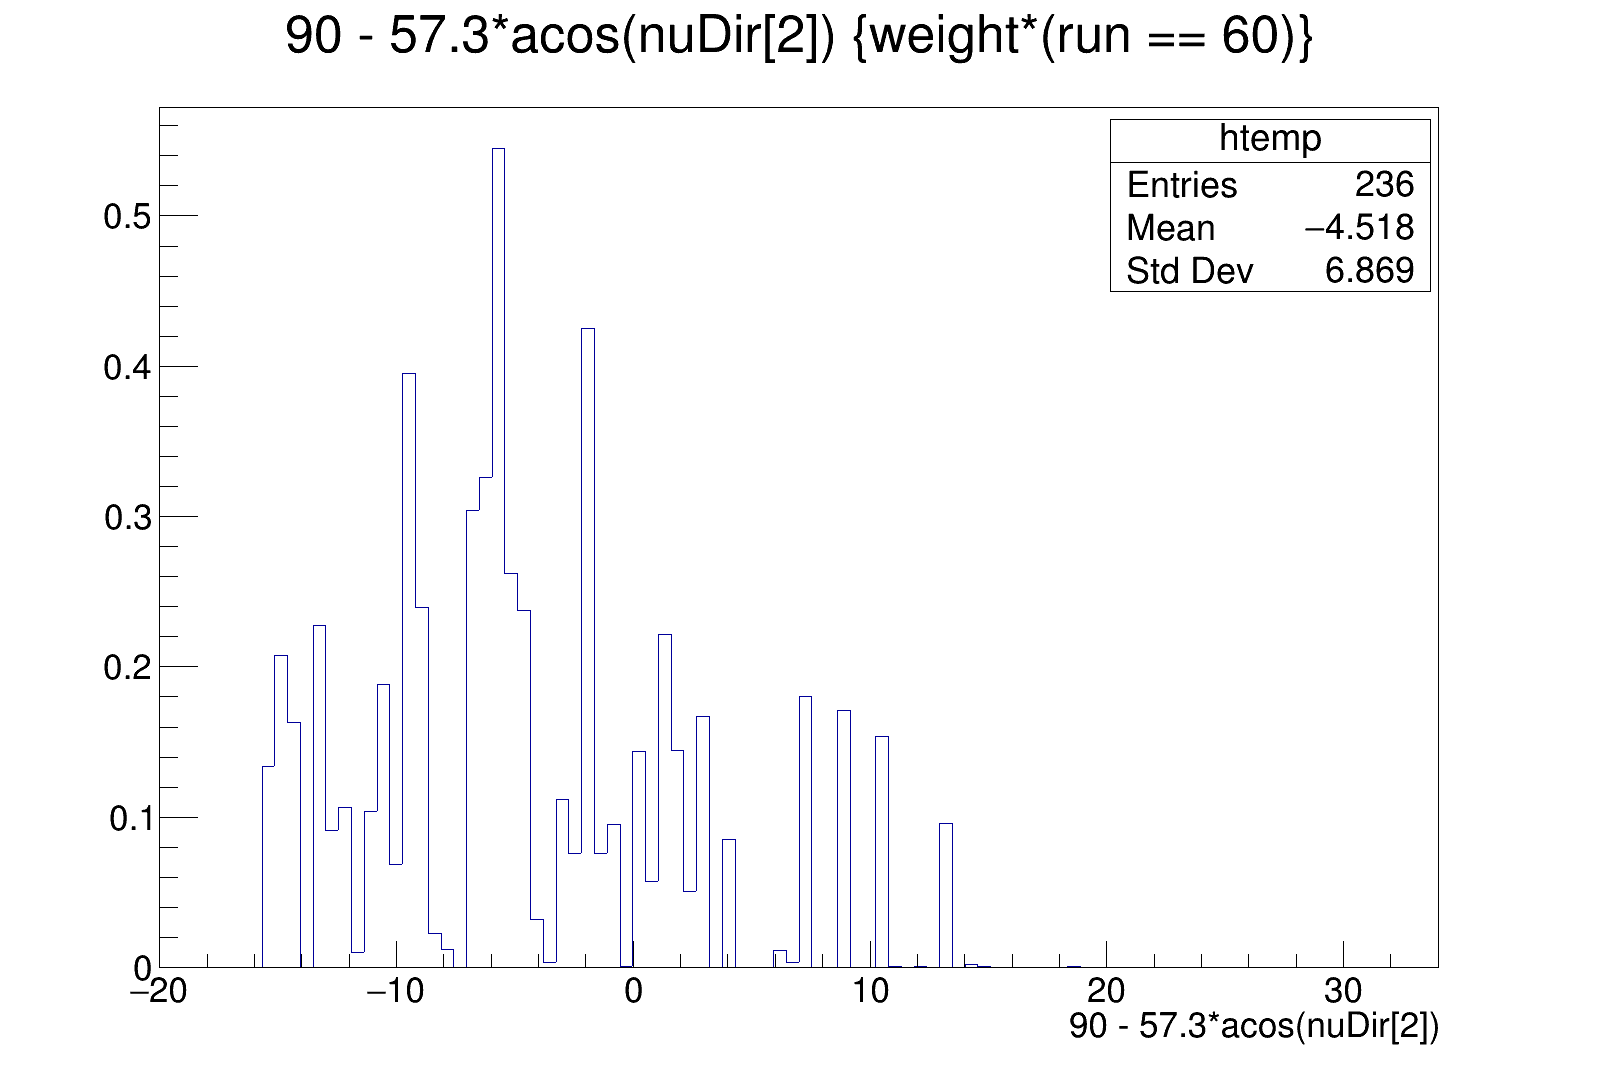
\includegraphics[width=.8\textwidth]{figures/koteraMarch30_acos_nuDir2_weighted.png}
\caption{Distribution of elevation angles of weighted simulated neutrinos using an isotropic Kotera flux. This distribution shows the allowed range of elevation angles of signals that ANITA can view as simulated by icemc.}
\label{nuDir_kotera_isotropic}
\end{figure}


\section{Sub-threshold search}

An important feature of a search involving transient sources such as \gls{grbs} is that analysis cuts or thresholds can be reduced as compared to the search for a diffuse flux of neutrinos. When searching for a diffuse flux of neutrinos, one has to search for neutrinos throughout the flight. In a diffuse search, we use 10\% of the data to set analysis cuts and search using the remaining 90\% data. Most of the data, whether it is the 10\% set or the 90\%, is noise or background events. The analysis cuts are set based on this huge amount of background. 

In contrast, \gls{grbs} take place at specific times, so the search for neutrinos from them can be constrained in time. A spatial direction is also associated with each \gls{grb}, therefore, the search can also be constrained in direction. When the search is constrained in time and/or direction, the dataset is dramatically reduced. Thus, the background levels in the search are automatically lowered. This allows us to set lower analysis cuts. In other words, a \gls{grb} search is a sub-threshold search. In the case of the binned analysis, the expectation is that a sub-threshold search will translate to lower LD cut values.

\subsection{Idea behind reduced LD cuts}

The idea behind lowering LD cuts for the \gls{grb} search as compared to the diffuse search is illustrated in Figure~\ref{reduced_ld}. Reducing the dataset by constraining the search in direction and/or time pushes the exponentially-falling distribution down as pictured with the down-pointing black arrow. Requiring the same number of background events to pass the LD cut pushes the cut to the left as pictured by the left-pointing black arrow. If the dataset is reduced by a factor F and the slope of the fit (solid red line) in Figure~\ref{reduced_ld} is given by $-b$ then the reduced LD cut is given by the relation in Equation~\ref{factor}. This relation is obtained by setting the background calculated using the diffuse LD cut, $cut_{old}$, equal to the background calculated using the \gls{grb} LD cut, $cut_{new}$. 


\begin{equation}
cut_{old} - cut_{new} = \frac{1}{b}\ln F
\label{factor}
\end{equation}


\begin{figure}
\centering
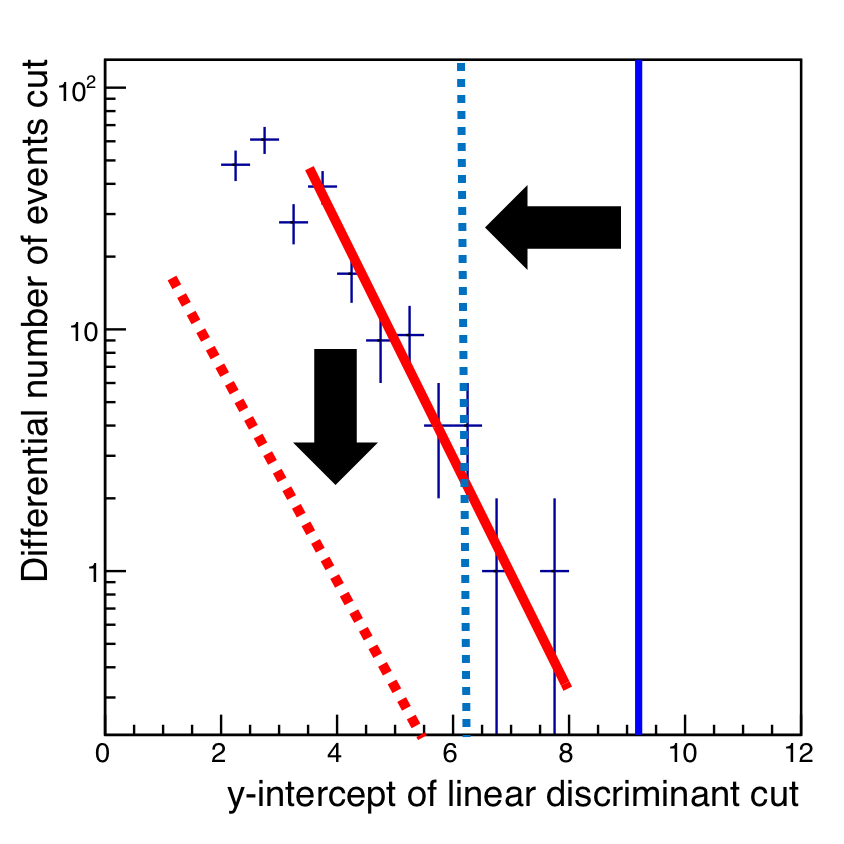
\includegraphics[width=0.9\textwidth]
{figures/reduced_ld.png}
\caption{Reducing the dataset by constraining in time and direction while allowing the same number of background events to pass the LD cut allows us to lower the cut. The shifts shown with solid black arrows here are not the actual shifts, but illustrations.}
\label{reduced_ld}
\end{figure}


\section{Constraining in direction and time}

Since \gls{grbs} are transient point sources, a search for neutrinos coming from \gls{grbs} can be constrained in time and direction. Both the time and direction associated with a \gls{grb} are available in the catalog as shown in Table~\ref{catalog}. Therefore, the data used to conduct the search for a neutrino from a \gls{grb} can be narrowed down based on this information. 


\subsection{Neutrino vs. RF direction}

The direction associated with a \gls{uhe} neutrino and the direction associated with the resulting \gls{rf} from that neutrino are not the same. Care must be taken to properly account for this difference in the elevation angle and azimuth associated with the \gls{grb} itself and the \gls{rf} signature of neutrinos from that \gls{grb}. 

The \gls{anita} simulation icemc can be used to calculate the difference between the neutrino direction and the \gls{rf} direction. In icemc, the neutrino direction, \gls{rf} direction, and payload position are given by the vectors shown using red arrows in the top part of Figure~\ref{getting_angles}. The elevation angle of the \gls{rf} as seen by the payload can be obtained via evaluation of the dot product of the \path{n_exit2bn[2]} vector (referred in short as \path{rf} in Figure~\ref{getting_angles}) and the \path{r_bn} vector. Similarly, the elevation angle of the neutrino as seen by the payload can be obtained by taking the dot product of the \path{nnu} vector with the \path{r_bn} vector. The difference in azimuthal angle associated with the \gls{rf} and the neutrino as seen by the payload can be obtained by first finding the components of \path{rf} and \path{nnu} that are perpendicular to \path{r_bn}, as shown in the bottom part of Figure~\ref{getting_angles}, and then taking their dot product. 

\begin{figure}
\centering
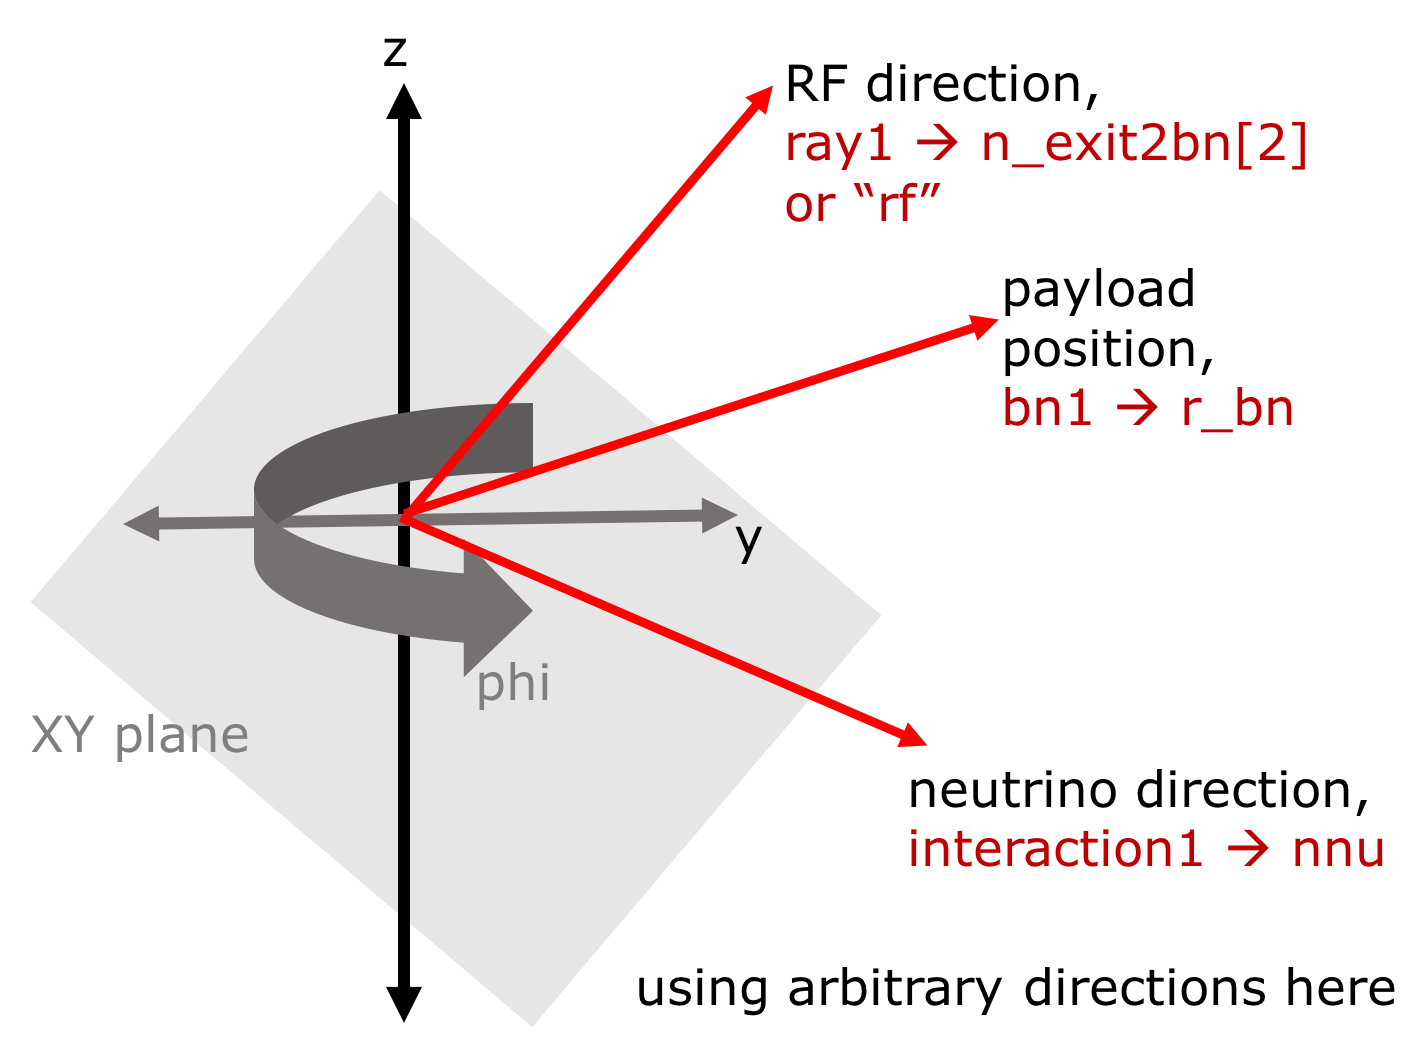
\includegraphics[width=0.8\textwidth]
{figures/getting_nnu_rf.png}
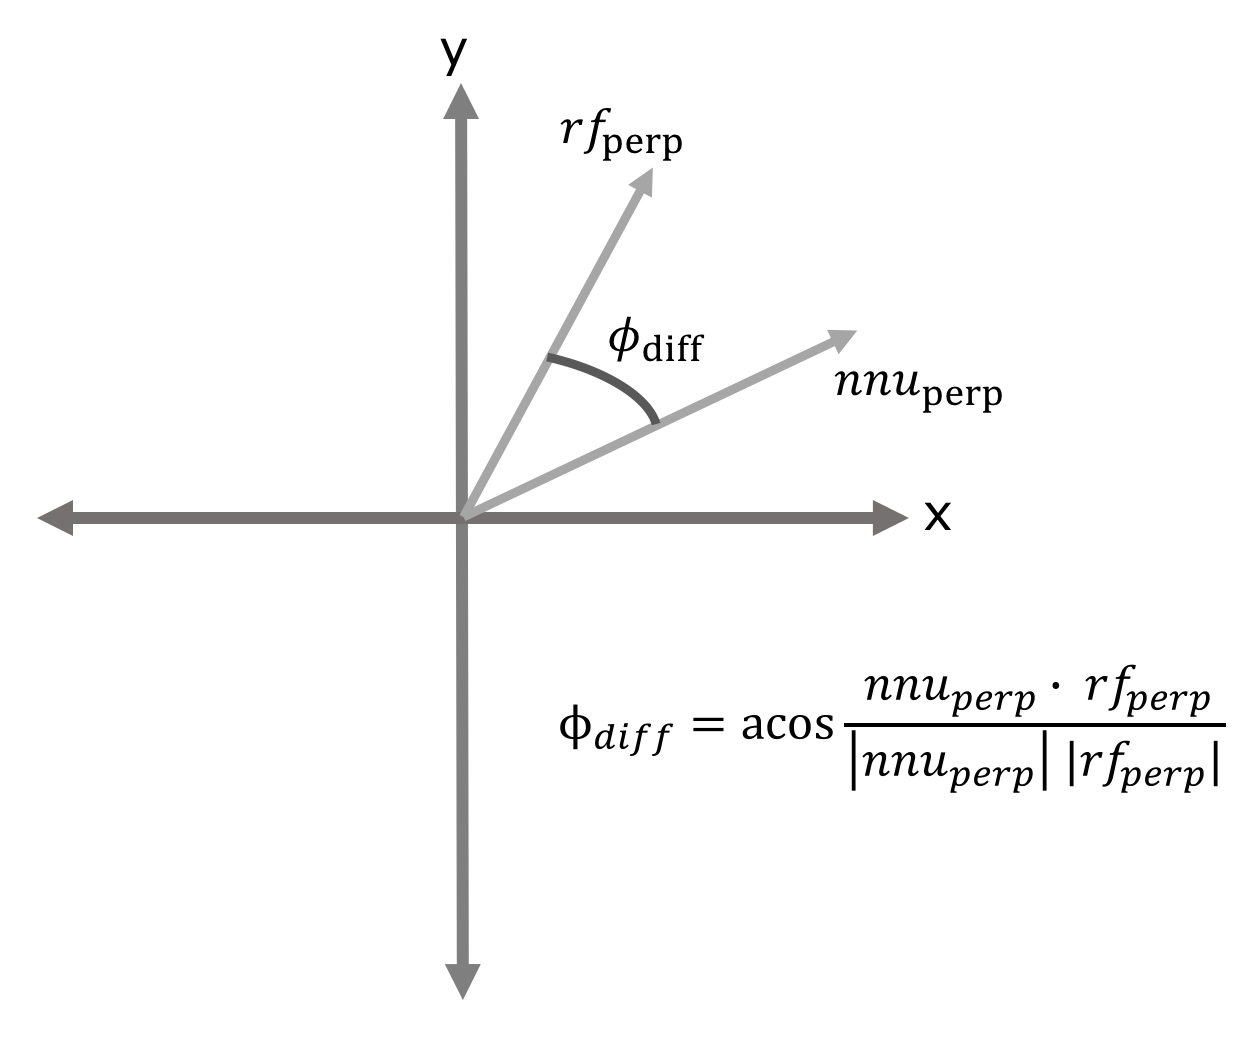
\includegraphics[width=0.8\textwidth]
{figures/rf_nnu_perp.png}
\caption{Visualization of angles involved in the calculation of the difference in elevation angle and azimuthal angle between neutrino and its associated RF direction. }
\label{getting_angles}
\end{figure}

Figure~\ref{angle_diff} shows a two-dimensional distribution of the difference in elevation angle (theta) and azimuthal angle (phi) as seen by the payload of the neutrino and \gls{rf} direction. This distribution is made with weighted simulated neutrinos that passed all triggers and were recorded as events in the \path{passing_events} tree in icemc. Note that icemc was run using the standard diffuse setting here so neutrinos thrown in the Monte Carlo would come from random directions, rather than a set source direction, however, the effect of seeing the \gls{rf} at a different direction than the corresponding neutrino direction is clearly seen here.  


\begin{figure}
\centering
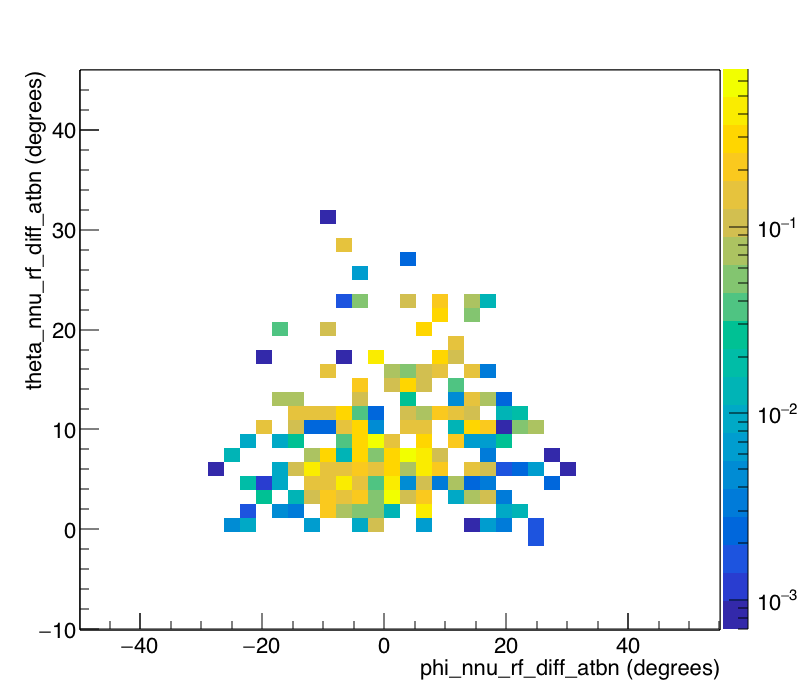
\includegraphics[width=0.9\textwidth]
{figures/phidiff_vs_thetadiff.png}
%\includegraphics[width=0.9\textwidth]
%{figures/theta_diff.png}
\caption{Two-dimensional distribution of the difference in elevation angle (theta) in the vertical axis and the difference in azimuthal angle (phi) in the horizontal axis of the neutrino and RF direction. All angles are as seen by the payload.}
\label{angle_diff}
\end{figure}


\subsection{Direction constraint}

Figure~\ref{angle_diff} helps to quantify the difference between the neutrino direction and the \gls{rf} direction. It is a two-dimensional distribution where color represents the number of weighted simulated neutrinos. The difference between the neutrino direction and the \gls{rf} direction in their azimuthal angle is shown along the horizontal axis. The difference in the elevation angle is shown in the vertical axis. The azimuthal angle difference has a spread between about -20 and 20 degrees, while the elevation angle goes from little under 0 degrees to about 30 degrees. 
Given this distribution, a conservative approach would be to do the search for neutrinos from a \gls{grb} in a patch of the sky covering about 1200 square degrees, that is, in a 30 degrees by 40 degrees area. Ideally, however, we would reduce the size of the search area in direction.  

As a first pass, for the direction constraint, 
data events with reconstructed azimuth within five degrees of the azimuth of each \gls{grb} were allowed to participate in the search. Meaning, if the azimuth associated with a \gls{grb} were to be 50 degrees, then events with reconstructed azimuth in the range of 45 - 55 degrees would be allowed in the search. In a second test, for the direction constraint in azimuth, data events with azimuth within 60 degrees of the azimuth of the \gls{grb} were allowed in the search. 
In both passes, no \gls{grb}-specific constraint on elevation angle was imposed on the data. The usual cut of allowing events with elevation angle in the range -6 to -35 degrees was in place. 

\subsection{Afterglows and time constraint}

The data allowed to participate in the \gls{grb} search should be constrained in time keeping the afterglow emission period of \gls{grbs} in mind. \gls{uhe} neutrinos are expected with higher probability during the afterglow emission of a \gls{grb}, as opposed to the prompt emission. \gls{grbs} are highly versatile, and both the prompt and afterglow periods can vary greatly from one \gls{grb} to another. The afterglow period, in particular, can be anywhere from a few minutes to days or even months. 

All \gls{grb} neutrino searches in the past have been constrained in time to no more than $10$ minutes. In this search, during the first test with five degree azimuth windows, the time was constrained to seven hours. When the azimuth window was widened to 60 degrees, the time was constrained to 45 minutes. This was to ensure that the number of events participating in the search in both cases is about the same so as to get similar reduced analysis thresholds. So if the direction window is widened the time window has to be shortened. Since there is a physics motivation (afterglows) to pursue searches in longer time windows, improving the constraint in direction is a suitable goal. 

\section{Blinding}

The search developed in this chapter is meant to be a blind analysis. 
%A blind search for \gls{grb} neutrinos was conducted using the \gls{anita}-3 data. 
Blinding means that all analysis cuts are determined using a subset of the data or a ``burn" sample that is not included in the actual search. In other words, there is a ``background region" and a ``signal region" of data. The background region is used for characterization of the background and determination of analysis cuts. The signal region is used to perform the actual search for a signal. In the diffuse search, a 10\% dataset is chosen as the background region and the remaining 90\% dataset is the signal region. Possible signal present in the signal region is not allowed to bias the analysis cuts and therefore, the search is blind. 

Blinding in the \gls{grb} search is similarly motivated as in 
the diffuse search, however, it is implemented differently. 
The \gls{grb} search, too, has a background region and a signal region. These are defined below. 

\subsection{Background region} 

Events from the 100\% \gls{anita}-3 dataset that were recorded in the chosen time window \textbf{before} the start of each \gls{grb} and having a reconstructed azimuth in the chosen azimuth window around the \gls{grb} are considered to be in the background region of each \gls{grb}. All of these events for all 18 \gls{grbs} taken together is the total background region of the search. Note that for a \gls{grb} search, we can use the 100\% dataset instead of only 10\% as in the diffuse search. Moreover, the background region is constrained in time and direction, also in contrast to the diffuse search. 

\subsection{Signal region}

Events from the 100\% \gls{anita}-3 dataset that were recorded in the chosen time window \textbf{after} the start of each \gls{grb} and having reconstructed azimuth in the chosen azimuth window around the azimuth of the \gls{grb} are considered to be in the signal region of each \gls{grb}. All of these events for all 18 \gls{grbs} taken together is the total signal region of the search. Again, note that the signal region of a \gls{grb} search is constrained in time and direction, automatically reducing the number of background events that would need to get cut by the analysis. 


\section{Binned analysis}

A search for \gls{grb} neutrinos was developed using the \gls{anita}-3 data following a variation of the binned analysis methods discussed in Chapters~\ref{analysis} and~\ref{results_diffuse}. In the binned analysis, the intended final cut is the LD cut. This cut is determined based on the distribution of y-intercepts of events in each geographical bin. Each distribution is fitted to an exponential function. The LD cut is optimized to produce the best limit on the chosen model of neutrino production. Details on the optimization process can be found in~\cite{brianDaileyThesis,samStaffordThesis,jacobGordonThesis}.

The search for \gls{grb} neutrinos in the \gls{anita}-3 data was performed after the completion of the search for a diffuse flux of neutrinos in the \gls{anita}-3 data. Therefore, the fundamental methods of the binned analysis were already developed to conduct a search. Adapting these methods to a \gls{grb} neutrino search involved certain modifications which we discuss in this section along with other details of the analysis.

\subsection{Combining bins}

Due to the time and direction constraints on the data participating in the \gls{grb} search, the overall dataset is greatly reduced. There are only $6860$ events in the background region of the \gls{grb} search compared to $82762$ events in the background region of the diffuse search, just before final cuts. Having fewer events in the background or signal region makes it challenging to have enough events in each bin to perform the binned analysis. Therefore, in the \gls{grb} search, certain bins were combined as necessary. 

Bins were combined only in the \gls{vpol} channel of the analysis. Bins with similar LD cuts in the diffuse search were combined as shown in Table~\ref{combine}. 

\begin{table}
\centering
\begin{tabular}{ |c|c|c| } 
\hline
Bin number & Diffuse LD cut & Combined bin number\\
\hline
2991 &	8.7 & \\
2997 &	9.3 & \\
2936 &	9.3 & 3010\\
3016 &	9.4 & \\
3010 &	9.4 & \\
\hline
2989 &	9.9 & \\
3030 &	9.9 & \\
3011 &	9.9 & 3013\\
3013 &	10 & \\
2990 &	10 & \\
\hline
3018 &	10.1 & \\
2988 &	10.1 & \\
2937 &	10.2 & 3018\\
2938 &	10.3 & \\
3008 &	10.4 & \\
\hline
2901 &	10.8 & \\
3015 &	10.9 & \\
3029 &	10.9 & \\
3014 &	11.0 & 3015\\
2971 &	11.1 & \\
3007 &	11.2 & \\
2977 &	11.2 & \\
\hline
2973 &	11.5 & \\
3004 &	11.7 & \\
2970 &	12.0 & \\
2939 &	12.1 & \\
2998 &	12.2 & 3012\\
3037 &	12.3 & \\
3012 &	12.5 & \\
2979 &	13.1 & \\
3019 &	13.5 & \\
\hline
2935 &	14.3 & \\
3003 &	14.4 & 3017\\
3017 &	14.6 & \\
\hline
\end{tabular}
\caption{Bins that were combined in the VPol channel. The number in the third column is the name given to the combined bin for that group. In practice, the events from each group of bins were treated as all belonging to the bin in the third column in order to combine the bins for the analysis.}
\label{combine}
\end{table}

\subsection{Distributions from the background region}

Events from the background region are processed through the different stages of the binned analysis. Before final cuts, distributions of y-intercepts of events are made for each bin. In the case of the \gls{vpol} analysis, bins are combined as shown in Table~\ref{combine} and distributions are made for the resulting combined bins. In the case of the \gls{hpol} analysis, bins are not combined and standard bins are used. These distributions are fitted to an exponential function. An optimized LD cut is chosen on the tail of each distribution and the background for that bin is estimated by integrating from the LD cut value to infinity.

At the stage of fitting the data in each bin to an exponential, some bins are lost. 
Bins that have less than five histogram bins with data or less than five events in the fit are not allowed to participate further in the analysis. Bins where the data cannot be fitted to an exponential or have a p-value less than 0.05 are lost as well. Distributions of data from the background region in the bins kept in the \gls{hpol} and \gls{vpol} channels and associated exponential fits are shown in Figures~\ref{hpol_expo} and~\ref{vpol_expo}.


\begin{figure}
\centering
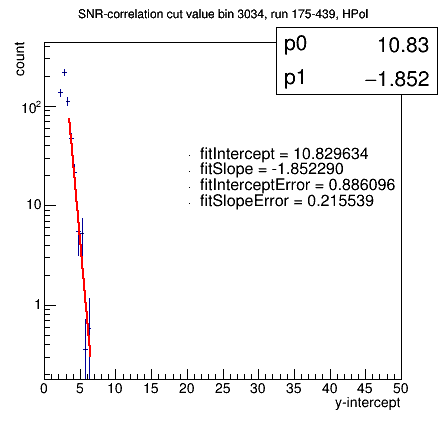
\includegraphics[width=.5\textwidth]
{figures/cutValHistH03034.png}
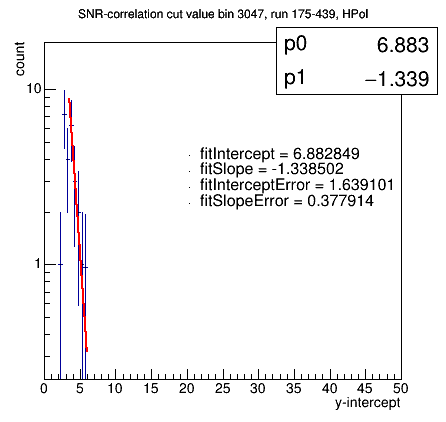
\includegraphics[width=.5\textwidth]
{figures/cutValHistH03047.png}
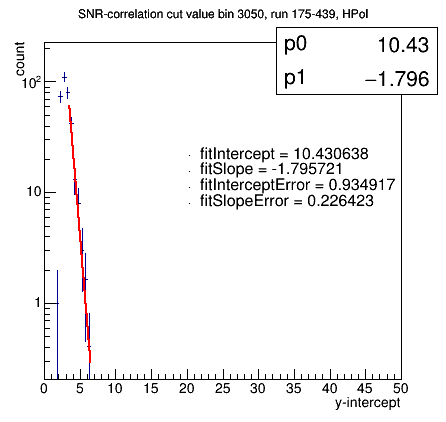
\includegraphics[width=.5\textwidth]
{figures/cutValHistH03050.png}
\caption{Distributions from the background region in bins kept in the HPol analysis.}
\label{hpol_expo}
\end{figure}


\begin{figure}
\centering
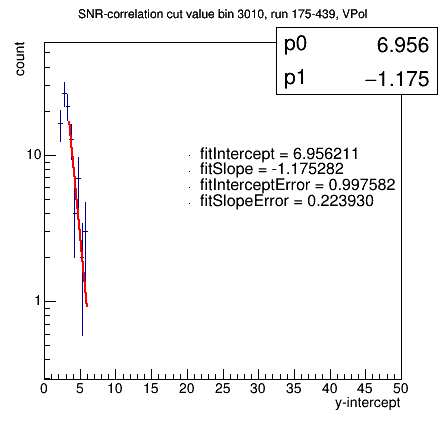
\includegraphics[width=.49\textwidth]
{figures/cutValHistV03010.png}
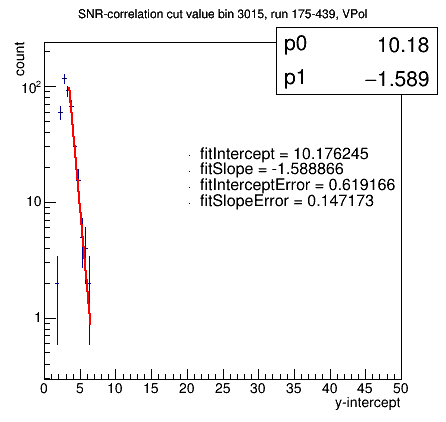
\includegraphics[width=.49\textwidth]
{figures/cutValHistV03015.png}
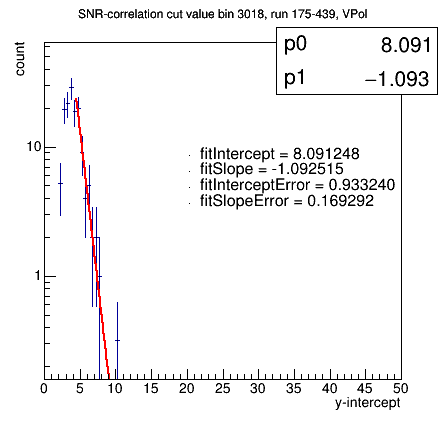
\includegraphics[width=.49\textwidth]
{figures/cutValHistV03018.png}
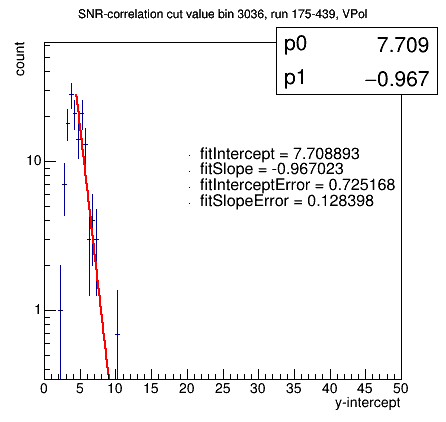
\includegraphics[width=.49\textwidth]
{figures/cutValHistV03036.png}
\caption{Distributions from the background region in bins kept in the VPol analysis.}
\label{vpol_expo}
\end{figure}


\subsection{Background estimates}

The number of background events estimated to pass the optimized LD cut in each bin is calculated by integrating the tail of the exponential fit in that bin from the LD cut value to infinity. The bin number, total events in the bin prior to the LD cut, p-value of the exponential fit, estimated background along with errors are shown for the \gls{hpol} and \gls{vpol} channel analyses in Table~\ref{hpol_table}. 

In the first pass, in the \gls{hpol} channel, three singlet bins were used. In the \gls{vpol} channel, three combined bins as well as one singlet bin was used. The singlet bin used in \gls{vpol} was not kept in the diffuse search due to having a p-value less than 0.05 in the diffuse search. In the second pass, in the \gls{hpol} channel, three singlet bins were used. In the \gls{vpol} channel, three combined bins and three singlet bins were used. Two of the singlet bins from this test were not kept in the diffuse search, again, due to p-value being less than 0.05 in that search. 

Note that the second pass was optimized using 100 pseudo-experiments to calculate the background estimates whereas the first pass was optimized using 5000. The background estimates are expected to be less accurate when fewer pseudo-experiments are performed. For the final optimization, it is recommended to use 5000 pseudo-experiments to calculate background estimates as was done for the diffuse search. 


\begin{table}
\centering
\begin{tabular}{ |c|c|c|c|c|c|c|c|c| } 
\hline
Bin & Pol & Total events & LD cut & p-value & Bg est & Bg Hi & Bg Lo & Diffuse LD cut\\
\hline
3034 & H & 548.1 & 6.9 & 0.7 & 0.30 & 0.46 & 0.22 & 9.1\\
3047 & H & 25.4 &	6.7	& 0.9 & 0.33 & 0.71 & 0.22 & 9.6\\
3050 & H & 333.0 & 6.8 & 0.9 & 0.36	& 0.57 & 0.27 & 13.7\\
\hline
\hline
\hline
3010 & V &	93.4  &	8.5 & 0.4 & 0.15 &	0.31 &	0.09 & 8.7 - 9.4\\
3015 & V &	393.5 &	8.1	& 0.9 & 0.17 &	0.25 &	0.13 & 10.8 - 11.2\\
3018 & V &	137.2 &	9.6 & 0.9 & 0.32 &	0.54 &	0.23 & 10.1 - 10.4\\
\hline
3036 & V &	133.8 &	11.7 &	0.1 &   0.11 &	0.19 &	0.07 & Bad p-value\\
\hline
\hline
\hline 
\hline
\hline
3034 & H & 149.6 & 8.8 & 0.9 & 0.48	& 0.86 & 0.35 & 9.1\\
3035 & H & 49.1 & 6.8 & 0.5 & 0.82 & 1.53 & 0.57 & 10.0\\
3050 & H & 122.9 & 8.5 & 0.8 & 0.20	& 0.33 & 0.14 & 13.7\\
\hline
\hline
\hline
3010 & V & 119.1 & 7.2 & 0.7 & 0.23	& 0.43 & 0.15 & 8.7 - 9.4\\
3015 & V & 625.9 & 9.3 & 0.7 & 0.41 & 0.58 & 0.33 & 10.8 - 11.2\\
3018 & V & 53.7	& 9.1 & 0.6	& 0.37	& 0.77 & 0.25 & 10.1 - 10.4\\
\hline
3021 & V & 144.8 & 13.1	& 0.65 & 0.69 & 1.00 & 0.52 & 26.24\\
3028 & V & 114.8 & 7.5 & 0.9 & 0.22	& 0.47 & 0.14 & Bad p-value\\
3036 & V & 111.9 & 7.8 & 0.9 & 0.44	& 0.77 & 0.30 & Bad p-value\\
\hline
\end{tabular}
\caption{Information on the GRB analysis in the HPol and VPol channels from two passes: top using smaller azimuth window and larger time window, bottom using larger azimuth window and smaller time window in the search. Bin numbers along with number of events in the bin, optimized LD cut, p-value of the exponential fit, background estimate along with errors, are shown. The right most column shows the LD cut for the bin in the diffuse search for comparison with the LD cut in the GRB search. Note that bins 3010, 3015, and 3018 were obtained by combining multiple bins.}
\label{hpol_table}
\end{table}


\subsection{LD cuts}

Table~\ref{hpol_table} shows the LD cuts for the different bins kept in the \gls{grb} search. 
The right most column of the table shows the LD cut value that was calculated for the bin or bins (in case of combining) in the diffuse search. This can be compared to the third column and seen that the LD cut calculated in the \gls{grb} search is always lower than the LD cut for the bin in the diffuse search. In case of the combined bins, the LD cut is always lower than the lowest LD cut associated with the bins used in combining. 

It would be pertinent to check whether the LD cuts have been lowered in the \gls{grb} search by the amount predicted by Equation~\ref{factor}, however, a few things must be kept in mind. It would only make sense to compare the LD cuts for the \gls{grb} vs. diffuse search for bins with similar distributions and exponential fits in both the \gls{grb} and diffuse search. In cases where bins had to be combined to conduct the \gls{grb} search this cannot be the case. Specifically, bins 3010, 3015, and 3018 are combined bins in the \gls{grb} search, taking data from multiple bins, so these combined bins cannot be compared to the singlet bins 3010, 3015, and 3018 in the diffuse search. Moreover, LD cuts should only be compared when the corresponding background estimate for the bin in both the \gls{grb} and diffuse search is the same. 

I checked for the case of bin 3034 in the \gls{hpol} channel and found that the difference in LD cuts according to Equation~\ref{factor} should be $4.7$. This is using $F$ of $2700$ and $b$ of $1.7$. The $b$ for the distribution for this bin in the \gls{grb} search is 1.8 and that in the diffuse search is 1.6, so I used $1.7$. The $2700$ comes from taking the ratio of the time for the whole flight over the time when signal is present ((22 days x 24 hours) / 7 hours) multiplied by the ratio of total azimuth over the chosen azimuth window (360 degrees / 10 degrees). The actual difference in the LD cuts, however, is $2.2$. It must be noted that the background estimates were not the same for this bin in the \gls{grb} vs. diffuse search, which is a requirement for Equation~\ref{factor} to be true.  
In the diffuse search, the background estimate was $0.36$ with a high error of $0.60$ and a low error of $0.24$. 
In the \gls{grb} search, the background estimate was $0.30$ with a high error of $0.46$ and a low error of $0.22$. 
For the final calculation, I would recommend checking that the backgrounds presented in Table~\ref{hpol_table} are not overestimated due to accounting for unnecessary systematic uncertainties. 


\section{Simulating neutrinos from a source direction}
\label{grb_sim}

In addition to applying analysis cuts to the data, all cuts are also applied to simulated neutrinos. This is done in order to determine the efficiency of the analysis and to set a limit on the chosen model of neutrino production, in the absence of a discovery. In order to perform an analysis to search for neutrinos from specific sources, rather than from all directions, it is necessary to have the capability to simulate neutrinos from those sources. Although \gls{anita} has had the capability to simulate a diffuse flux of \gls{uhe} neutrinos, there was not yet a method in place to simulate neutrinos from specified sources. 

\subsection{Overview of icemc}

The \gls{anita} simulation package is known as icemc. This is maintained on GitHub at this link: \href{https://github.com/anitaNeutrino/icemc}{https://github.com/anitaNeutrino/icemc}. It mainly consists of several classes, such as, the \path{Primaries}, \path{balloon}, \path{ray}, and \path{icemodel} classes and a main executable code called \path{icemc}. The executable code \path{icemc} contains a Monte Carlo algorithm. Inside \path{icemc}, all the classes are instantiated and associated functions are called. Settings such as the number of neutrinos to throw in the Monte Carlo, the energy of neutrinos, which \gls{anita} flight, can be initialized using an inputs file, for example, the \path{inputs.anita3.conf} file associated with the \gls{anita}-3 simulation.  

Inside \path{icemc}, there is a for loop over \path{NNU}, the number of neutrinos specified in the inputs file. Cuts are applied at different stages to the neutrinos that don't meet the criteria to be observable by \gls{anita}. Cuts are implemented with the command \path{continue}, that is, the code skips to the next neutrino in the loop when there is a cut. The first set of \path{continues} are shown in Figure~\ref{first_continues}.

The main functions that are called in the loop and their purpose are briefly described below. 


\subsubsection{PickBalloonPosition}

This is a function in the \path{balloon} class. It picks the balloon position and at the same time sets the masks and thresholds. 

\subsubsection{PickDownwardInteractionPoint}

This is a function in the \path{balloon} class. 
It sets the interaction point in the ice. 

\subsubsection{GetSurfaceNormal}

This is a function in the \path{ray} class. 
It finds the normal to the surface taking into account the tilt from the differential heights between neighboring bins. 

\subsubsection{GetRFExit}

This is a function in the \path{ray} class. 
At this stage, Snell's law is used to get the first guess at the
direction of the \gls{rf} as it leaves ice surface.
The starting guess was to use the direction that is simply radially outward from interaction position. This now takes into account the balloon position and the surface normal.

\subsubsection{GetDirection}

This is a function written in \path{icemc.cc}. 
It picks a neutrino direction such that its Cerenkov cone is close enough to the balloon line of sight that we have a ``chance in hell" of seeing the signal.


\subsubsection{GetViewAngle}

This is a function written in \path{icemc.cc}. 
It finds the angle between the ray and the neutrino direction.


\subsubsection{WhereDoesItEnter}

This is a function in the \path{earthmodel} class. 
It finds the neutrino entry point. 

\subsubsection{Getchord}

This is a function in the \path{earthmodel} class. It finds the length of the chord through the earth that the neutrino would have had to travel. 

\subsubsection{IsAbsorbed}

This is a function in \path{icemc.cc}. 
It takes the best case scenario chord length and finds the corresponding weight of the neutrino. 

\subsubsection{GetVmMHz}

This is a function in the \path{signal} class. 
It finds the magnitude of the signal. 

\subsubsection{TaperVmMHz}

This is a function in the \path{signal} class. 
It applies the angular dependence of the signal. The difference between the ``viewangle" and the Cerenkov angle is multiplied by the signal to account for the fast fall-off from being on-cone. 


\begin{figure}
\centering
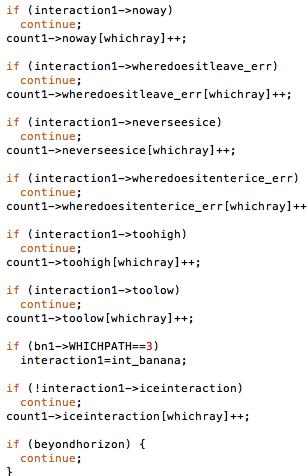
\includegraphics[width=0.8\textwidth]
{figures/icemc_first_continues.png}
\caption{The first set of cuts on neutrinos thrown in the Monte Carlo.}
\label{first_continues}
\end{figure}

\subsection{Source mode}

A source mode was developed in icemc for the purpose of running it for neutrinos coming from a specified source.
A setting was added to the \path{Settings} class to make a source mode which when turned on in the \path{inputs} file, switches icemc to the source mode.
In the source mode, the neutrino direction, \path{nnu}, is set using an addition to the function \path{GetDirection}. Additionally, a new function called \path{PickGrbDirection} has been added to the \path{Primaries} class. 

Tests of the source mode are shown in Figure~\ref{source_tests}. The top two plots are made with the source setting on, that is, by setting the neutrino direction to a specific vector: (-1,0,0) on the left and (1,0,0) on the right. There is no time constraint in the top plots. The bottom plot is made by imposing a time constraint of 6 hours in addition to setting \path{nnu} to (1,0,0). An outline of Antarctica is shown in these plots in blue and the \gls{anita}-3 flight path in red. The black dots are simulated neutrinos that passed the trigger. 

The positions of the black dots shown in Figure~\ref{source_tests} are consistent with the neutrinos coming from a source on the left (top left plot) and from the right (top right plot), however, it is apparent that no neutrino passed on the right side of the continent in the top left plot. Upon investigating the cause of nothing passing on the right side, it was found that \path{count1->nchanceinhell2} was an order of magnitude smaller on the right side than on the left side of the continent. Therefore, the cut just before \path{count1->nchanceinhell2} is counted was investigated and it was verified that the quantity, ``chance", in short, being checked against the threshold in this cut was also smaller on the right side. The distributions for ``chance" on the right and left side are shown by the top plots of Figure~\ref{debug}. The quantity \path{Tools::dMax(vmmhz, Anita::NFREQ)} within ``chance" is the one responsible for ``chance" being smaller, as verified from its distributions. 
The term ``chance" here is used to denote in short the following expression in \path{icemc}. 

\begin{center}
``chance" $=$ 
\path{settings1->CHANCEINHELL_FACTOR*Tools::dMax(vmmhz, Anita::NFREQ)*heff_max*0.5*(anita1->bwmin/1.E6)}
\end{center}

\begin{figure}
\centering
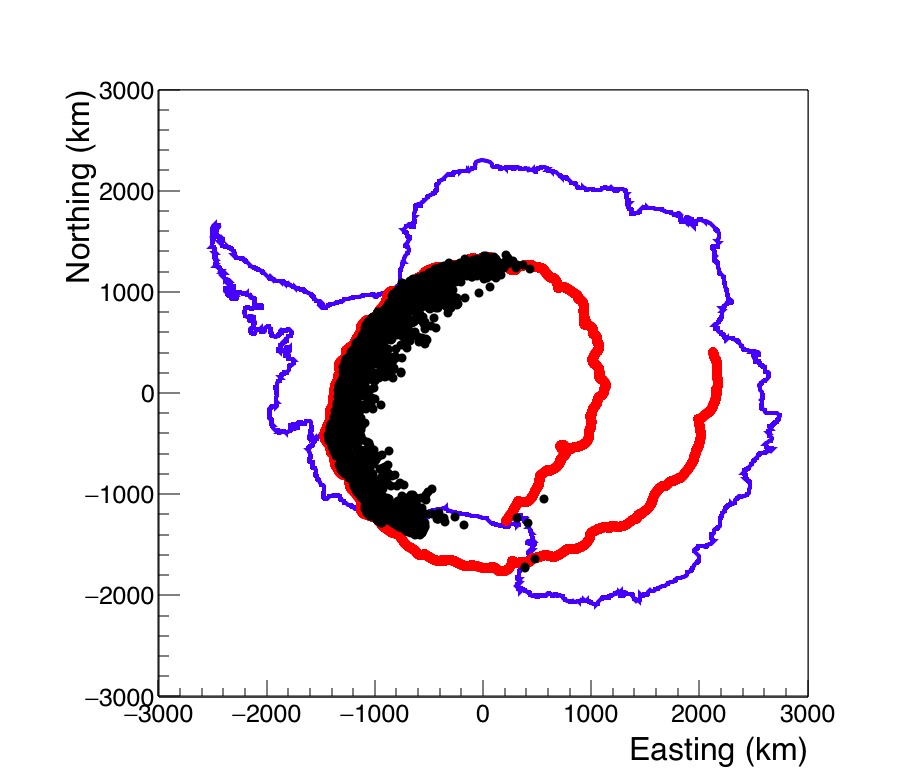
\includegraphics[width=.49\textwidth]{figures/source_test_using_nnu-100.png}
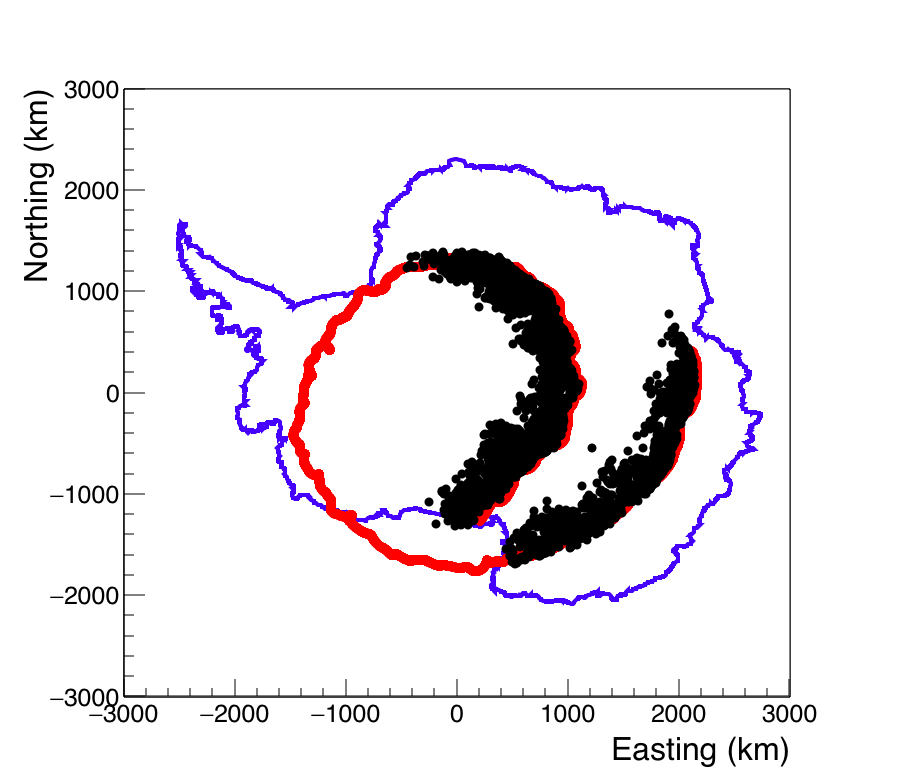
\includegraphics[width=.49\textwidth]
{figures/source_test_using_nnu100.png}
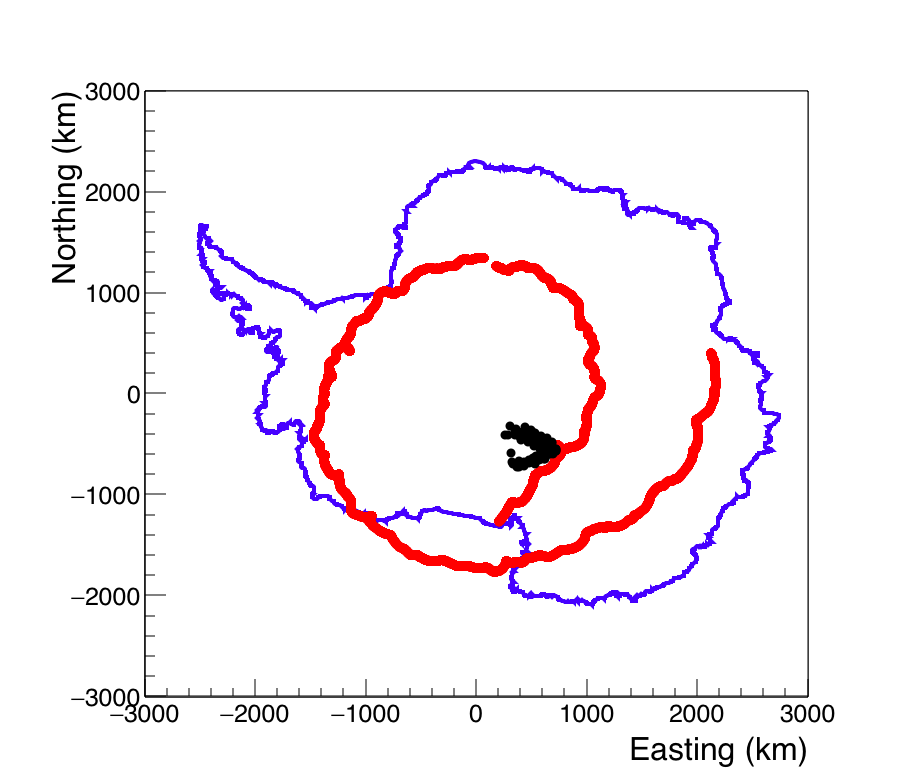
\includegraphics[width=.49\textwidth]
{figures/source_test_using_nnu100_time_cut_6hrs.png}
\caption{Tests of the source setting in icemc. The figure on the top left shows simulated neutrinos using neutrino direction vector (-1,0,0) and top right using neutrino direction vector (1,0,0). The figure on the bottom shows simulated neutrinos with an additional constraint on time. The bottom figure is for a source emitting neutrinos for 6 hours.}
\label{source_tests}
\end{figure}

The earliest place in the code where the distribution for \path{Tools::dMax(vmmhz, Anita::NFREQ)} is different for right versus left was investigated. 
It was found that it was different before and after the function \path{TaperVmMHz}, which has several inputs, including \path{viewangle}. 
It was found that the variable \path{viewangle} was different for the left versus right side as shown by the bottom distributions of Figure~\ref{debug}. This variable is set in a function in \path{icemc.cc} called \path{GetViewAngle}. This function takes \path{nnu} as an input, and was examined for any possible errors. No error was found, however, it was noted that the quantity \path{viewangle} was being calculated by taking the dot product of two vectors, \path{nnu} and \path{nrf2_iceside} and then finding the acosine, resulting in the angle returned being indistinguishable from its negative. 

\begin{figure}
\centering
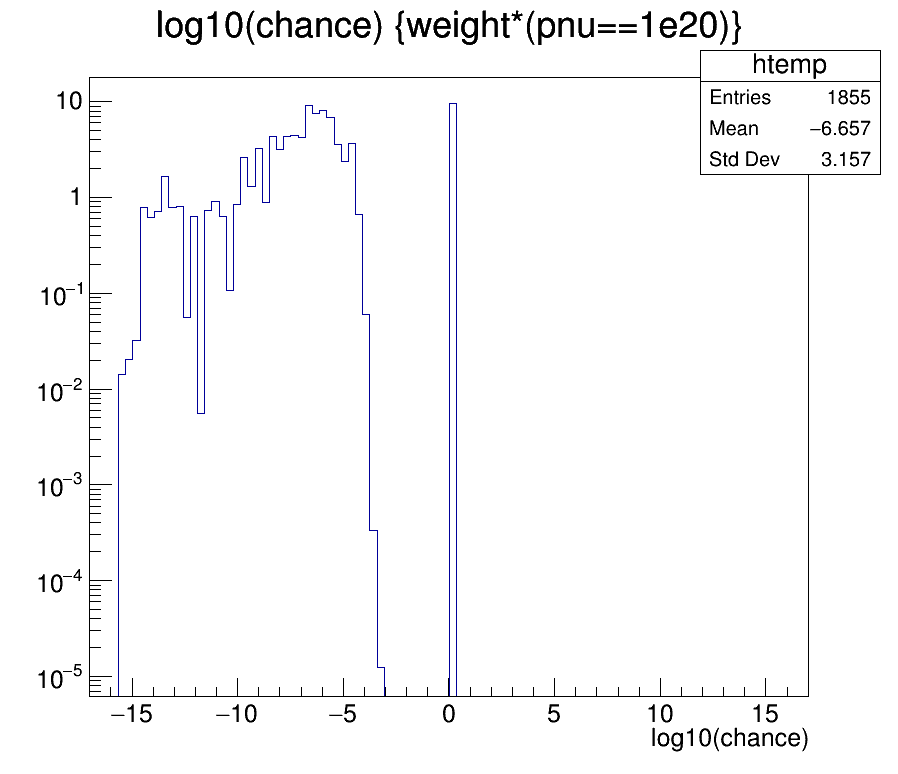
\includegraphics[width=.49\textwidth]{figures/chance_leftside_left.png}
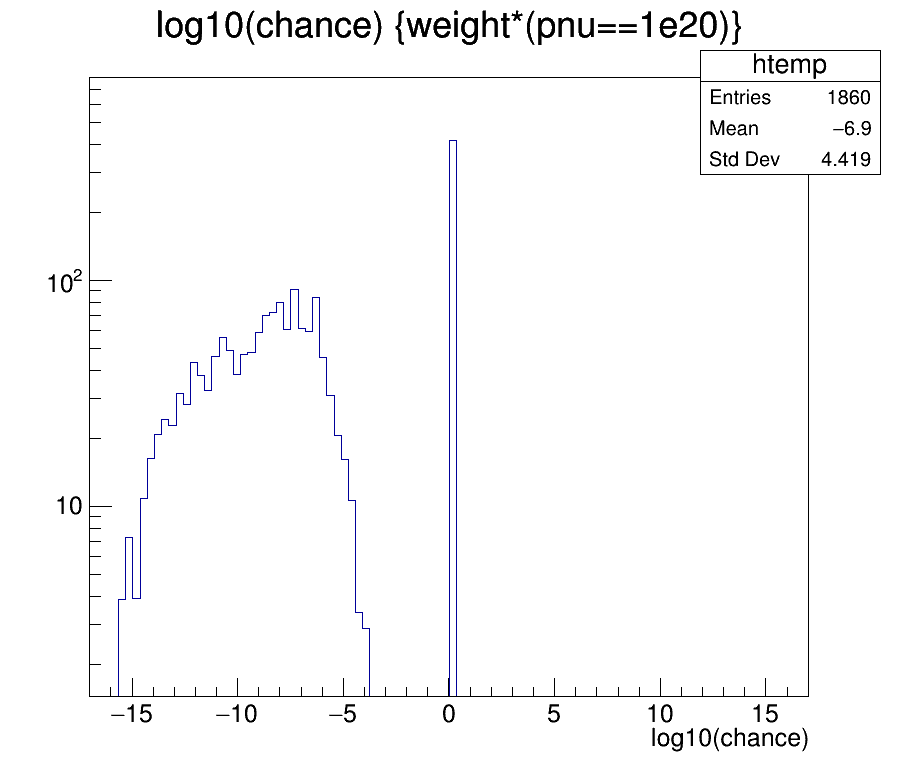
\includegraphics[width=.49\textwidth]
{figures/chance_leftside_right.png}
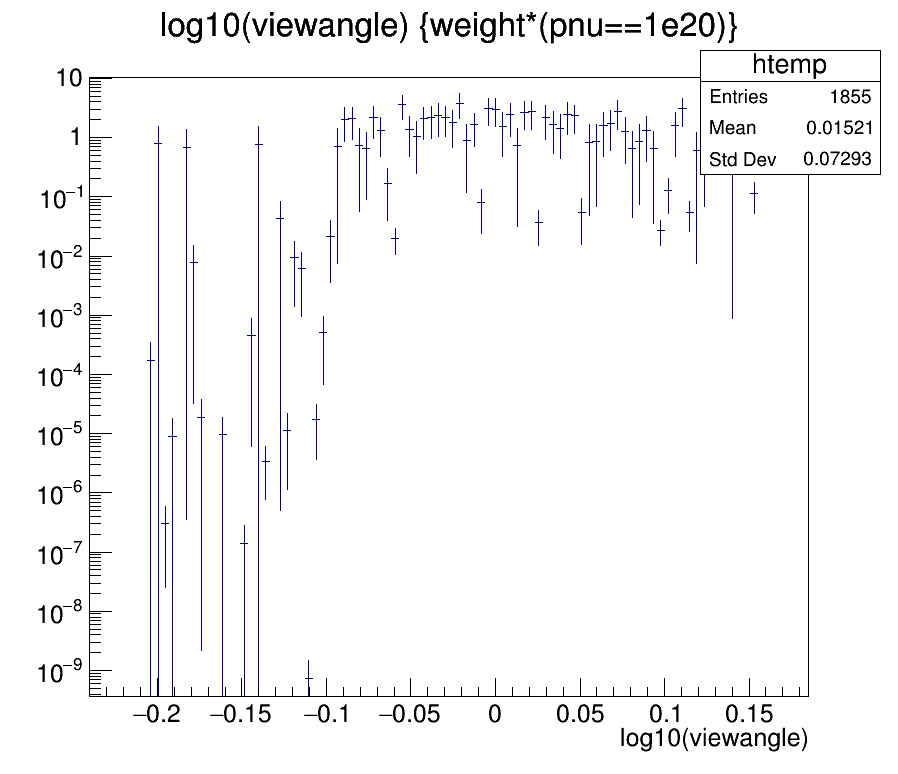
\includegraphics[width=.49\textwidth]
{figures/taper_viewangle_left.png}
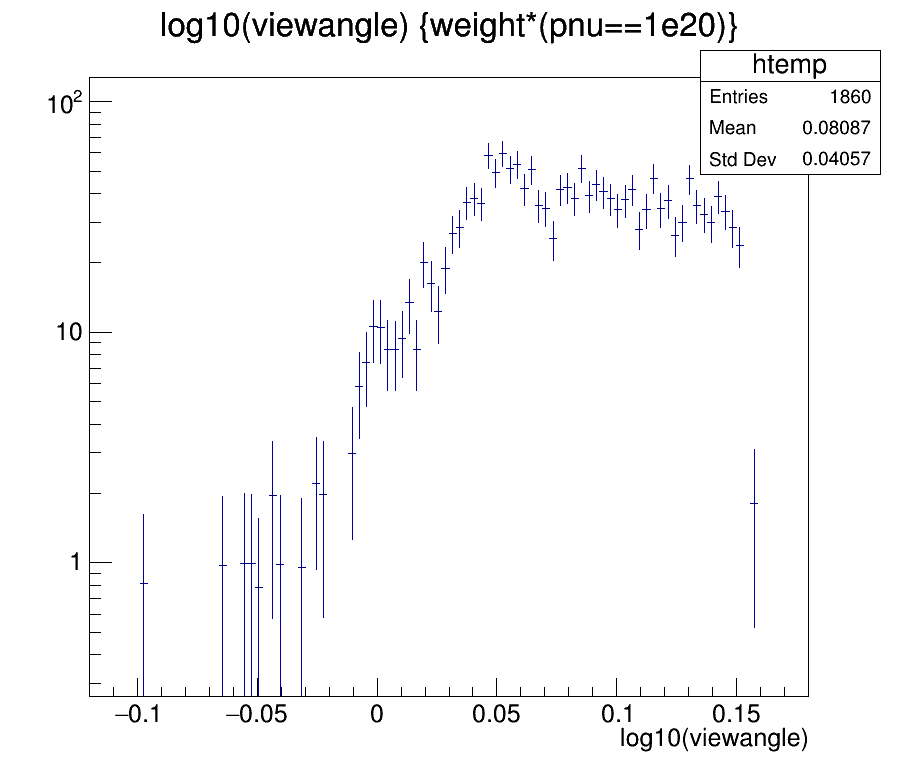
\includegraphics[width=.49\textwidth]
{figures/taper_viewangle_right.png}
\caption{Distributions showing differences in the values of quantities calculated for simulated neutrinos on the left (left) and right (right) side of the continent.}
\label{debug}
\end{figure}
